\chapter{Testing \& Evaluation}

A known limitation of the system is that there is no user-friendly way of defining the dimensions of the CA simulator. That being said, to test the rules' accuracies and how well the simulation scales, some changes need to be made to the code base at the lower level. 
\\ \\
The scalability of the simulator is tested as the simulator size is dependent on the size of the computer screen. No performance enhancements will be made, as only the display size will be changed. 
\section{Simulation Scaling Test}
Before going to the details on the procedure of this test, it is important to understand how the program determines the dimensions of the two-dimensional array for the simulator. This is discussed in \ref{2darr_creator}.
We measure how well the simulation scales by measuring the amount of time taken between each generation's transition, i.e. how long it takes for the simulator to apply the transition rules to all the cells, and the average time taken to do so. The average time taken to transition between ten generations is the dependent variable. The independent variable will be a coefficient introduced to the resolution, as the size of the simulator is determined in the \texttt{setup()} function where the rows and column count are divided by the resolution. Only the code from the \texttt{sketch.js} file are changed to support logging. The following changes are introduced to the system to evaluate its scalability:
\begin{enumerate}
    \item A new Array \texttt{times\_10} will be made to store the times taken for transition between 10 generations.
    \item A new floating point number, \texttt{coeff} to be multiplied to the resolution in the \texttt{setup} function.
    \item The \texttt{draw()} function will automatically stop after ten iterations, then log the times taken. 
\end{enumerate}
The rules operated in this test will be the CGOL and Forest Fire Simulator Rules.
\newpage
\noindent It is important to note that the number of rows and columns for the grid are directly proportional to the resolution coefficient, as shown in the table below and the graph that follows:
\begin{table}[H]
\begin{tabular}{|c|c|c|}
\hline
\begin{tabular}[c]{@{}c@{}}Resolution \\ Coefficient\end{tabular} & Rows & Cols \\ \hline
1                                                                 & 60   & 96   \\ \hline
1.5                                                               & 90   & 144  \\ \hline
2                                                                 & 120  & 192  \\ \hline
2.5                                                               & 150  & 240  \\ \hline
3                                                                 & 180  & 288  \\ \hline
3.5                                                               & 210  & 336  \\ \hline
4                                                                 & 240  & 384  \\ \hline
4.5                                                               & 270  & 432  \\ \hline
\end{tabular}
\caption{Table of Resolution Coefficient to Rows and Columns}
\end{table}
\begin{figure}[H]
    \caption{Graph showing of Resolution Coefficient vs. no. of Rows and Columns}
    \centering
    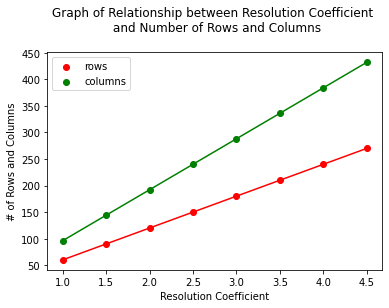
\includegraphics[scale=0.70]{linear_rows_cols.png}
\end{figure}
\noindent That being said, this section will observe the relationship between the coefficient (inherently the number of rows and columns) and the time it takes to apply the transition rules:
\begin{center}
\begin{table}[H]
\begin{tabular}{|c|cccccccccc|c|}
\hline
\begin{tabular}[c]{@{}c@{}}Resolution \\ Coefficient\end{tabular} & \multicolumn{10}{c|}{Generation Transition Times (ms)} & Average (ms) \\ \hline
1                                                                 & \multicolumn{1}{c|}{61}   & \multicolumn{1}{c|}{40}   & \multicolumn{1}{c|}{39}   & \multicolumn{1}{c|}{39}   & \multicolumn{1}{c|}{39}   & \multicolumn{1}{c|}{30}   & \multicolumn{1}{c|}{31}   & \multicolumn{1}{c|}{31}   & \multicolumn{1}{c|}{31}   & 32   & 37.3         \\ \hline
1.5                                                               & \multicolumn{1}{c|}{105}  & \multicolumn{1}{c|}{116}  & \multicolumn{1}{c|}{109}  & \multicolumn{1}{c|}{92}   & \multicolumn{1}{c|}{90}   & \multicolumn{1}{c|}{91}   & \multicolumn{1}{c|}{92}   & \multicolumn{1}{c|}{95}   & \multicolumn{1}{c|}{95}   & 95   & 98           \\ \hline
2                                                                 & \multicolumn{1}{c|}{548}  & \multicolumn{1}{c|}{564}  & \multicolumn{1}{c|}{559}  & \multicolumn{1}{c|}{498}  & \multicolumn{1}{c|}{508}  & \multicolumn{1}{c|}{506}  & \multicolumn{1}{c|}{507}  & \multicolumn{1}{c|}{509}  & \multicolumn{1}{c|}{465}  & 493  & 517.7        \\ \hline
2.5                                                               & \multicolumn{1}{c|}{645}  & \multicolumn{1}{c|}{609}  & \multicolumn{1}{c|}{626}  & \multicolumn{1}{c|}{552}  & \multicolumn{1}{c|}{595}  & \multicolumn{1}{c|}{586}  & \multicolumn{1}{c|}{623}  & \multicolumn{1}{c|}{552}  & \multicolumn{1}{c|}{590}  & 561  & 593.9        \\ \hline
3                                                                 & \multicolumn{1}{c|}{1434} & \multicolumn{1}{c|}{1307} & \multicolumn{1}{c|}{1254} & \multicolumn{1}{c|}{1209} & \multicolumn{1}{c|}{1213} & \multicolumn{1}{c|}{1156} & \multicolumn{1}{c|}{1169} & \multicolumn{1}{c|}{1174} & \multicolumn{1}{c|}{1180} & 1146 & 1224.2       \\ \hline
3.5                                                               & \multicolumn{1}{c|}{1876} & \multicolumn{1}{c|}{1759} & \multicolumn{1}{c|}{1790} & \multicolumn{1}{c|}{1923} & \multicolumn{1}{c|}{1822} & \multicolumn{1}{c|}{1748} & \multicolumn{1}{c|}{1703} & \multicolumn{1}{c|}{1786} & \multicolumn{1}{c|}{1686} & 1663 & 1775.6       \\ \hline
4                                                                 & \multicolumn{1}{c|}{2345} & \multicolumn{1}{c|}{1802} & \multicolumn{1}{c|}{1855} & \multicolumn{1}{c|}{1891} & \multicolumn{1}{c|}{1810} & \multicolumn{1}{c|}{1794} & \multicolumn{1}{c|}{1772} & \multicolumn{1}{c|}{1786} & \multicolumn{1}{c|}{1820} & 1954 & 1882.9       \\ \hline
4.5                                                               & \multicolumn{1}{c|}{3070} & \multicolumn{1}{c|}{2946} & \multicolumn{1}{c|}{3059} & \multicolumn{1}{c|}{2835} & \multicolumn{1}{c|}{2805} & \multicolumn{1}{c|}{2738} & \multicolumn{1}{c|}{2792} & \multicolumn{1}{c|}{2824} & \multicolumn{1}{c|}{2735} & 2644 & 2844.8       \\ \hline
\end{tabular}
\caption{Table of Resolution Coefficient and Generation Transition Times for CGOL Rules in ms}
\end{table}
\end{center}
\noindent From the table above, it can be seen that there is a positive correlation between the resolution coefficient and the average time taken for the transition to occur to the entirety of the CA grid. The same experiment can be done for the forest fire simulator rules. The results are provided in the table below:
\begin{table}[H]
\begin{tabular}{|c|cccccccccc|c|}
\hline
\begin{tabular}[c]{@{}c@{}}Resolution \\ Coefficient\end{tabular} & \multicolumn{10}{c|}{Generation Transition Times (ms)}                                                                                                                                                                                                           & Average (ms) \\ \hline
1                                                                 & \multicolumn{1}{c|}{45}   & \multicolumn{1}{c|}{22}   & \multicolumn{1}{c|}{23}   & \multicolumn{1}{c|}{26}   & \multicolumn{1}{c|}{27}   & \multicolumn{1}{c|}{28}   & \multicolumn{1}{c|}{24}   & \multicolumn{1}{c|}{23}   & \multicolumn{1}{c|}{40}   & 24   & 28.2         \\ \hline
1.5                                                               & \multicolumn{1}{c|}{93}   & \multicolumn{1}{c|}{98}   & \multicolumn{1}{c|}{76}   & \multicolumn{1}{c|}{81}   & \multicolumn{1}{c|}{80}   & \multicolumn{1}{c|}{72}   & \multicolumn{1}{c|}{80}   & \multicolumn{1}{c|}{92}   & \multicolumn{1}{c|}{76}   & 82   & 83.0         \\ \hline
2                                                                 & \multicolumn{1}{c|}{524}  & \multicolumn{1}{c|}{466}  & \multicolumn{1}{c|}{564}  & \multicolumn{1}{c|}{510}  & \multicolumn{1}{c|}{453}  & \multicolumn{1}{c|}{508}  & \multicolumn{1}{c|}{495}  & \multicolumn{1}{c|}{464}  & \multicolumn{1}{c|}{446}  & 478  & 490.8        \\ \hline
2.5                                                               & \multicolumn{1}{c|}{592}  & \multicolumn{1}{c|}{613}  & \multicolumn{1}{c|}{523}  & \multicolumn{1}{c|}{559}  & \multicolumn{1}{c|}{551}  & \multicolumn{1}{c|}{588}  & \multicolumn{1}{c|}{547}  & \multicolumn{1}{c|}{545}  & \multicolumn{1}{c|}{592}  & 566  & 567.6        \\ \hline
3                                                                 & \multicolumn{1}{c|}{1250} & \multicolumn{1}{c|}{1185} & \multicolumn{1}{c|}{1266} & \multicolumn{1}{c|}{1149} & \multicolumn{1}{c|}{1158} & \multicolumn{1}{c|}{1159} & \multicolumn{1}{c|}{1117} & \multicolumn{1}{c|}{1134} & \multicolumn{1}{c|}{1108} & 1084 & 1161.0       \\ \hline
3.5                                                               & \multicolumn{1}{c|}{1718} & \multicolumn{1}{c|}{1728} & \multicolumn{1}{c|}{1795} & \multicolumn{1}{c|}{1724} & \multicolumn{1}{c|}{1709} & \multicolumn{1}{c|}{1640} & \multicolumn{1}{c|}{1647} & \multicolumn{1}{c|}{1586} & \multicolumn{1}{c|}{1678} & 1591 & 1681.6       \\ \hline
4                                                                 & \multicolumn{1}{c|}{2029} & \multicolumn{1}{c|}{2188} & \multicolumn{1}{c|}{2294} & \multicolumn{1}{c|}{1850} & \multicolumn{1}{c|}{1901} & \multicolumn{1}{c|}{1799} & \multicolumn{1}{c|}{1896} & \multicolumn{1}{c|}{1886} & \multicolumn{1}{c|}{1800} & 1881 & 1952.4       \\ \hline
4.5                                                               & \multicolumn{1}{c|}{2551} & \multicolumn{1}{c|}{2658} & \multicolumn{1}{c|}{2552} & \multicolumn{1}{c|}{2547} & \multicolumn{1}{c|}{2509} & \multicolumn{1}{c|}{2511} & \multicolumn{1}{c|}{2520} & \multicolumn{1}{c|}{2545} & \multicolumn{1}{c|}{2575} & 2748 & 2571.6       \\ \hline
\end{tabular}
\caption{Table of Resolution Coefficient and Generation Transition Times for Forest Fire Simulator Rules in ms}
\end{table}
\noindent The curve below visualizes the relationship between the resolution coefficient and the average transition time from one generation to another. 
\begin{figure}[H]
    \caption{Graph showing of Resolution Coefficient vs. Avg. Transition Times}
    \centering
    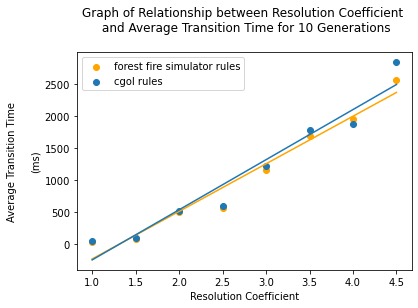
\includegraphics[scale=0.70]{plot_res_ttime.png}
\end{figure}
\noindent Based on the straight line and minimal signs of deviation, there is evidently a direct proportional relationship between the resolution coefficient and the average transition times. This is because the growth in number of rows and columns is directly proportional to the growth of the resolution coefficient. 

\newpage
\section{User Acceptance Testing}
In order to obtain feedback from users about this system's perceived usefulness, a qualitative interview was conducted. Two one-on-one interviews were conducted at different sittings. Both interview participants were computer science students at the University of Manchester. Each participant has also indicated familiarity with JSON and CAs (only CGOL). 
\\ \\
No personally identifiable data is collected during the interview. Both participants have indicated their consent in participating by signing a form, and are aware that participation is entirely voluntary and could withdraw from the interview at any point. 
\subsection{Setup and Methodology}
A document was created to act as a guide for the interviewees. This document was to be shown side-by-side the software in hand (see Appendix \ref{appendix:questionnaire}). Additionally, the Think Aloud method was adopted throughout the interview process. This means that the participants continuously spoke aloud any words that appear in their mind as they complete the tasks, and even up until concluding the interview \cite{charters2003thinkaloud}. I as the researcher was present beside the participant(s) to observe each of their thought processes, take notes, and provide support if required. 
\\ \\
Before conducting the interviews, one line of the code was changed. This change resulted in the radio button that populated the rules editor with the Map Generation CA (bottom left) to be hidden. This will prevent the participant in enabling the Map Generation CA rules, as the interview will involve the process of replicating the aforementioned rules (final part of Appendix \ref{appendix:questionnaire}). The Appendix also serves as the questions asked throughout the interview.

\subsection{Understanding the User Interface}
This part of the interview involved identifying the rule editor, simulator, and the buttons (Appendix \ref{appendix:questionnaire}). None of the interviewees experienced difficulties in identifying the visible components of the software. Both participants completed this part relatively quickly.
\\ \\
However, both participants showed a slight difficulty in detecting the buttons. A suggestion that was given would be to increase the sizes of the buttons at the very top, or move them downwards to increase visibility. 
\subsection{Understanding the Rules}
In this part, at the same sitting, three sets of tasks relating to the JSON-format rules were given to the participants. The aims of each tasks are given below, in addition to their results. See the more detailed step-by-step instructions in the Appendix \ref{appendix:questionnaire}.
\newpage
\subsubsection{Color Changing}
This section required the participants to change the color of the 'dead' state from CGOL, from black to red. 
\\ \\
Both participants found this step to be relatively trivial as both simply had to look for the value in the JSON rules that represents a color (in this case-black), and simply replaced it to the required 'red' color. 

\subsubsection{Changing the Totalistic Transition Rules}
The participants were required in this section to make changes to the rules of CGOL by starting with the default settings. In general, both participants showed some signs of difficulty in understanding how the rules worked, despite having been exposed to JSON and CAs.  
\\ \\
The first participant took less time to complete this task when compared to the second participant, though admitted it was considerably harder than the previous task as they (first participant) had to spend time understanding how the rules worked first. The second participant commented that "getting past the conditionals was the hardest part". They (second participant) however concluded that after understanding how the conditionals worked, working around it was quite simple. 
\\ \\
It is important to note that both participants at this stage have still not gone through the rules guide. Both participants tried to understand how the rules worked by comparing the English translation of the CA's rules to system-defined format. 

\subsubsection{Changing the Probabilistic Transition Rules} \label{probabilistic_test}
In this part, participants were tasked to interface with the forest fire propagation rules and simulator. Upon starting this task, both participants had to follow a specific set of steps to set up the system for the forest fire simulation environment. This setup process took slightly longer than I initially expected it to be. I ended up providing hints and explicit guidance on the procedure to set up the rules before moving on to the main bit of the forest fire propagation CA.
\\ \\
Both participants showed intrigue in the forest fire propagation rules when it was running. The first task in this part (aside from setting up) was to infer what the rules in the editor meant. Both participants understood the total-probabilistic rules (\texttt{total-p}) a bit faster than previous. Additionally, both participants have at this stage started consulting the documentation. This resulted in the second task being completed much faster than expected. However, the final task was considerably harder for both. 
\newpage
\subsubsection{Replicating the 2D Map Generation Rules based on Provided Specifications}
This final part of the interview required both participants to replicate the Game Development Map Generation rules (specified in Appendix \ref{appendix:gamedevmap_rules}) from the CGOL rules (specified in Appendix \ref{appendix:default_cgol}). In summary, both participants successfully completed this task and replicated the 2D Map Generation Rules as specified. 
\\ \\
Starting from the CGOL default rules, both participants took the same approach of deleting the \texttt{0} key entirely, replacing the colors, and resorted only to using the \texttt{default} key. Both understood the specifications, but were slightly baffled at how the rules implemented the specifications given. More on this in the following section.

\subsection{Analysis and Participant Suggestions} \label{analysis_suggestions}
Firstly, there was a general confusion on whether which state number corresponded to what number. In the case of CGOL, the states of \textbf{Dead} and \textbf{Alive} were assigned state numbers \textbf{0} and \textbf{1} respectively. This was not made clear in the beginning, and the confusion was present in the preceding tasks. When modifying the forest fire rules, the first participant looked at the \texttt{colors} key in the \texttt{\$\_meta} object and inferred the relationship between state names and numbers. A similar observation was done by the same participant when interacting with the forest fire CA rules - correlating the colors red, green, and black to fire, vulnerable vegetation, and burnt/invulnerable entities. Both participants, however suggested adding a descriptor field in the rules, to make it easier to identify which numbers corresponded to which states. 
\\ \\
Both participants showed signs of confusion when preparing the system to simulate the forest fire CA rules (subsection \ref{probabilistic_test}). This confusion was followed by a suggestion from both participants, to remove the 'number of states' text area and integrate that information to the dynamic rules \texttt{\$\_meta} tag. 
\\ \\
As the issues mentioned in the two paragraphs previous are relatively straightforward to implement, I've mentioned how this could be implemented in the \textbf{Potential Extension Work} section (\ref{potential_extension_work}) in the next chapter.
\\ \\
When interfacing with both the totalistic and total-probabilistic type of rules, the \texttt{total} argument caused confusion for both participants. As a result, I pointed both participants to the help page for the rules. They both noted as well that individually listing integers when it comes to describing the totalistic rules were somewhat impractical. An example of this would be how the 2D Map Generation rules were specified (see in section \ref{gamedevimp}) and how they were translated as rules supplied to the system. When the specifications state "less than or equal to four neighbours", the rules write \texttt{[0, 1, 2, 3, 4]} and checks if the number of neighbours is in that array.
\\ \\
Additional suggestions that were made included syntax highlighting and auto-indentation. Furthermore, both participants quoted that learning and interacting with JSON on-the-spot was a rather daunting experience. 